% ------------------------------------------------------------------------------
% Este fichero es parte de la plantilla LaTeX para la realización de Proyectos
% Final de Grado, protegido bajo los términos de la licencia GFDL.
% Para más información, la licencia completa viene incluida en el
% fichero fdl-1.3.tex

% Copyright (C) 2012 SPI-FM. Universidad de Cádiz
% ------------------------------------------------------------------------------

Esta sección cubre el análisis del sistema de información a desarrollar, haciendo uso del lenguaje de modelado UML.

\section{Modelo Conceptual}
A partir de los requisitos de información, se desarrollará un diagrama conceptual de clases UML. En ella identificaremos las clases, atributos y relaciones entre ellas tal y como podemos ver en la figura \ref{fig:digclases}.

\begin{figure}[!hpt]
	\begin{center} 
		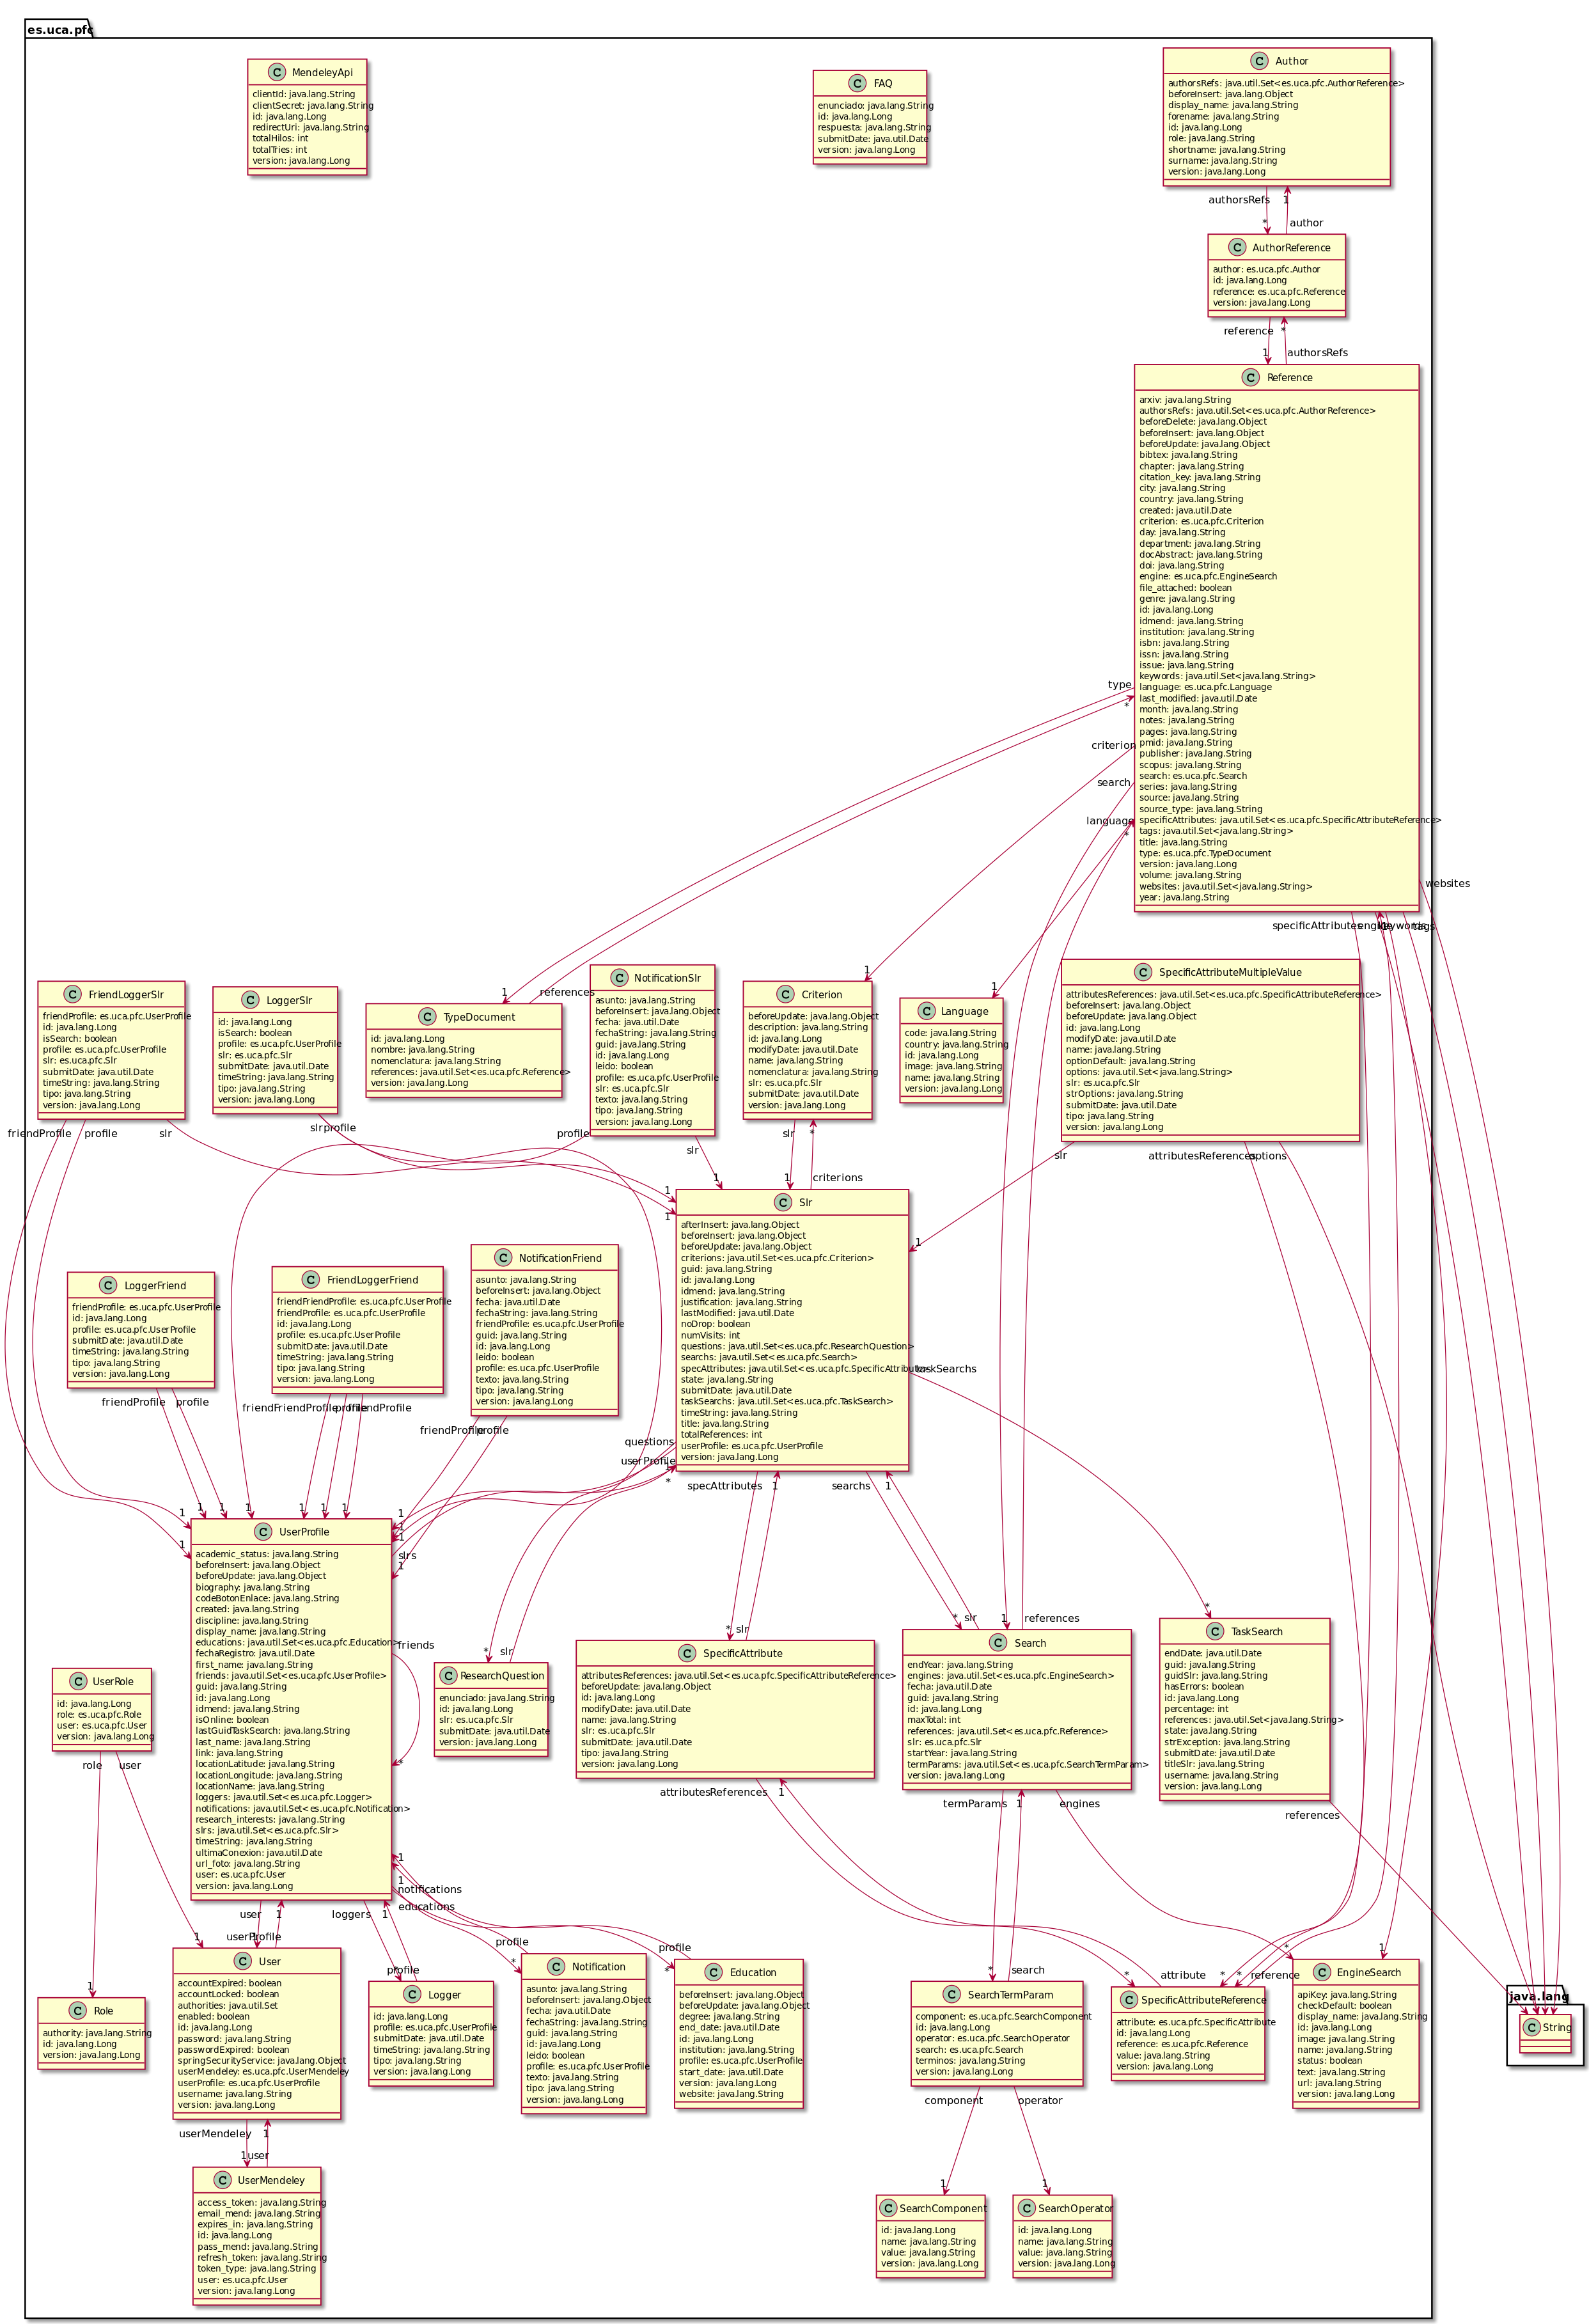
\includegraphics[width=\linewidth]{class-diagram.png}
		\caption{Diagrama conceptual de clases UML.}
		\label{fig:digclases}
	\end{center}
\end{figure}

%A partir de los requisitos de información, se desarrollará un diagrama conceptual de clases UML, identificando las clases, atributos, relaciones, restricciones adicionales y reglas de derivación necesarias.

\section{Modelo de Casos de Uso}
A partir de los requisitos funcionales descritos en apartados anteriores, se emplearan los casos de uso como mecanismo para representar las interacciones entre los actores y el sistema a desarrollar.
%A partir de los requisitos funcionales descritos anteriormente, se emplearan los casos de uso como mecanismo para representar las interacciones entre los actores y el sistema bajo estudio. Para cada caso de uso deberá indicarse los actores implicados, las precondiciones y postcondiciones, los pasos que conforman el escenario principal y el conjunto de posibles escenarios alternativos.

\subsection{Actores} 
Los diferentes roles que con el sistema pueden interactuar son los siguientes:

\begin{itemize}
	\item Investigador. Esta figura representa el usuario principal del sistema web. Una persona con este rol podrá realizar revisiones sistemáticas de la literatura y efectuar todas las tareas relacionadas con ellas.
	\item Administrador. Esta figura podrá realizar todas las funciones del rol investigador, junto con el mantenimiento de gestión de los usuarios y los errores de búsquedas de referencias bibliográficas producidas en el sistema.
\end{itemize}

%En este apartado se describirán los diferentes roles que juegan los usuarios que interactúan con el sistema. Los actores pueden ser roles de personas físicas, sistemas externos o incluso el tiempo (eventos temporales).

\subsection{Diagramas y especificación de casos de uso}
En esta sección se mostrarán los diagramas de casos de uso de la aplicación web (\ref{fig:cu01}, \ref{fig:cu02}, \ref{fig:cu03}, \ref{fig:cu04}, \ref{fig:cu05}, \ref{fig:cu06}, \ref{fig:cu07}, \ref{fig:cu08}), así como la especificación de los mismos mediante escenarios de casos de uso tal y como describimos en las tablas correspondientes a cada caso de uso.

\begin{figure}[hp!]
	\begin{center} 
		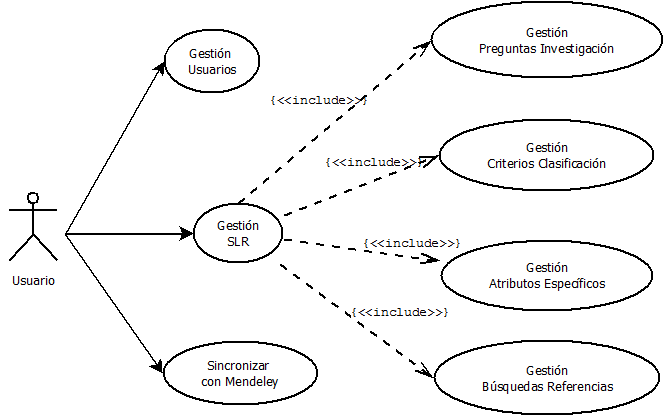
\includegraphics[scale=0.5]{cu-sistema.png}
		\caption{Diagrama casos de usos del sistema.}
		\label{fig:cu01}
	\end{center}
\end{figure}

\begin{figure}[hp!]
	\begin{center} 
		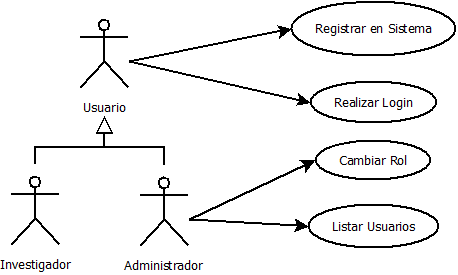
\includegraphics[scale=0.6]{cu-gestusuarios.png}
		\caption{Diagrama casos de usos de la gestión de usuarios.}
		\label{fig:cu02}
	\end{center}
\end{figure}

\begin{figure}[hp!]
	\begin{center}
		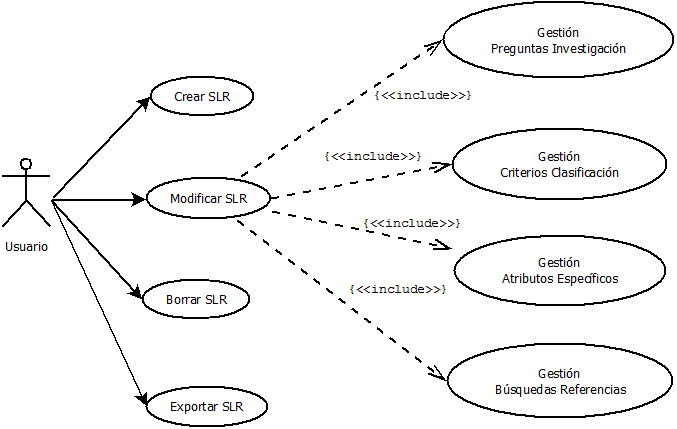
\includegraphics[scale=0.55]{cu-gestslr.png}
		\caption{Diagrama casos de usos de la gestión de revisiones sistemáticas.}
		\label{fig:cu03}
	\end{center}
\end{figure}

\begin{figure}[hp!]
	\begin{center}
		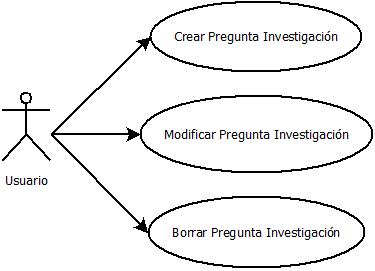
\includegraphics[scale=0.55]{cu-gestpreginv.png}
		\caption{Diagrama casos de usos de la gestión de preguntas de investigación.}
		\label{fig:cu04}
	\end{center}
\end{figure}

\begin{figure}[hp!]
	\begin{center}
		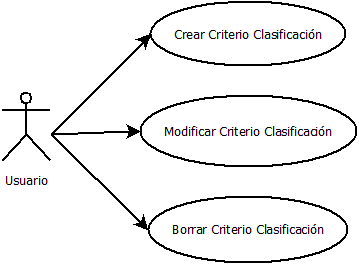
\includegraphics[scale=0.55]{cu-gestcrit.png}
		\caption{Diagrama casos de usos de la gestión de criterios de clasificación.}
		\label{fig:cu05}
	\end{center}
\end{figure}

\begin{figure}[hp!]
	\begin{center}
		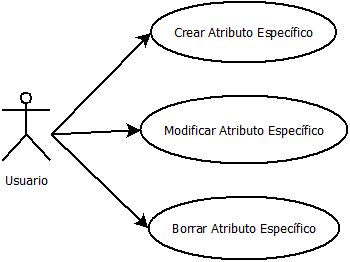
\includegraphics[scale=0.55]{cu-gestatesp.png}
		\caption{Diagrama casos de usos de la gestión de atributos específicos.}
		\label{fig:cu06}
	\end{center}
\end{figure}

\begin{figure}[hp!]
	\begin{center}
		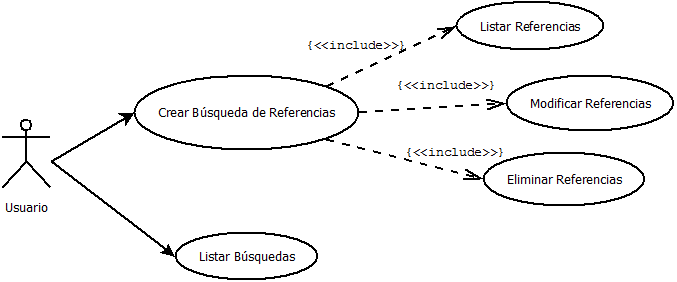
\includegraphics[scale=0.55]{cu-gestbusquedas.png}
		\caption{Diagrama casos de usos de la gestión de búsquedas de referencias bibliográficas.}
		\label{fig:cu07}
	\end{center}
\end{figure}

\newpage

\begin{figure}[hp!]
	\begin{center}
		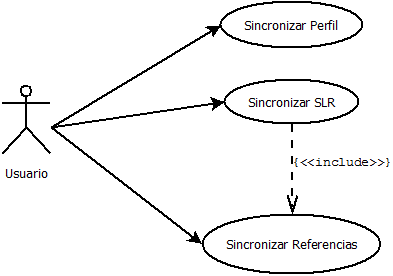
\includegraphics[scale=0.55]{cu-sincromend.png}
		\caption{Diagrama casos de usos de la sincronización con Mendeley.}
		\label{fig:cu08}
	\end{center}
\end{figure}

\begin{table}[!hbt]
	\begin{center}
		\begin{tabular}{|p{4cm}|p{11cm}|}
			\hline
			\textbf{Nombre} & CU-01 Registrar en sistema\\
			\hline
			\textbf{Descripción} & El usuario se registra en el sistema por primera vez para poder crear revisiones sistemáticas de la literatura.\\
			\hline
			\textbf{Precondición} & El usuario tiene una cuenta de Mendeley y no se ha logado antes en el sistema.\\
			\hline
			\textbf{Postcondición} & El usuario tiene acceso a la aplicación web.\\
			\hline
			\textbf{Actores} & Usuario\\
			\hline
			\textbf{Escenario principal} & 
				\begin{enumerate}
					\item El usuario introduce el email y contraseña de la cuenta Mendeley.
					\item El sistema valida que el email y la contraseña sean correctas redirigiendo al usuario a la pantalla principal de la aplicación web.
				\end{enumerate}
			\\
			\hline
			\textbf{\shortstack[l]{Escenarios \\ alternativos}} & 
				
				\begin{enumerate}[label=2 \alph*]
					%\setcounter{enumi}{2}
					\item El sistema verifica que el email y la contraseña no son correctas. Volvemos al paso 1.
				\end{enumerate}
			\\
			\hline
		\end{tabular}
		\caption{CU-01 Registar en sistema}
		\label{table:cu01}
	\end{center}
\end{table}

\begin{table}[!hbt]
	\begin{center}
		\begin{tabular}{|p{4cm}|p{11cm}|}
			\hline
			\textbf{Nombre} & CU-02 Realizar login\\
			\hline
			\textbf{Descripción} & El usuario se identifica en el sistema web.\\
			\hline
			\textbf{Precondición} & El usuario debe estar registrado en el sistema web.\\
			\hline
			\textbf{Postcondición} & El usuario tiene acceso a la aplicación web.\\
			\hline
			\textbf{Actores} & Usuario\\
			\hline
			\textbf{Escenario principal} & 
				\begin{enumerate}
					\item El usuario introduce el email y contraseña de la cuenta Mendeley.
					\item El sistema valida que el email y la contraseña sean correctas redirigiendo al usuario a la pantalla principal de la aplicación web.
				\end{enumerate}
			\\
			\hline
			\textbf{\shortstack[l]{Escenarios \\ alternativos}} & 
				
				\begin{enumerate}[label=2 \alph*]
					%\setcounter{enumi}{2}
					\item El sistema verifica que el email y la contraseña no son correctas. Volvemos al paso 1.
				\end{enumerate}
			\\
			\hline
		\end{tabular}
		\caption{CU-02 Realizar login}
		\label{table:cu02}
	\end{center}
\end{table}

\begin{table}[!hbt]
	\begin{center}
		\begin{tabular}{|p{4cm}|p{11cm}|}
			\hline
			\textbf{Nombre} & CU-03 Cambiar rol\\
			\hline
			\textbf{Descripción} & El administrador del sistema puede cambiar de rol a otro usuario.\\
			\hline
			\textbf{Precondición} & El usuario debe estar logado en el sistema y poseer rol administrador.\\
			\hline
			\textbf{Postcondición} & El administrador cambiar de rol a otro usuario.\\
			\hline
			\textbf{Actores} & Administrador\\
			\hline
			\textbf{Escenario principal} & 
				\begin{enumerate}
					\item El administrador del sistema busca al usuario a través de su email.
					\item El sistema ofrece toda la información del usuario.
					\item El administrador selecciona la opción de cambiar de rol al usuario.
					\item El sistema realiza el cambio y muestra un mensaje de que el proceso se ha realizado correctamente.
				\end{enumerate}
			\\
			\hline
			\textbf{\shortstack[l]{Escenarios \\ alternativos}} & --
			\\
			\hline
		\end{tabular}
		\caption{CU-03 Cambiar rol}
		\label{table:cu03}
	\end{center}
\end{table}

\begin{table}[!hbt]
	\begin{center}
		\begin{tabular}{|p{4cm}|p{11cm}|}
			\hline
			\textbf{Nombre} & CU-04 Listar Usuarios\\
			\hline
			\textbf{Descripción} & El administrador puede obtener una lista de todos los usuarios registrados en la aplicación web.\\
			\hline
			\textbf{Precondición} & El administrador está logado en el sistema y tiene rol administrador.\\
			\hline
			\textbf{Postcondición} & El administrador obtiene un listado completo de los usuarios registrados en el sistema.\\
			\hline
			\textbf{Actores} & Administrador\\
			\hline
			\textbf{Escenario principal} & 
				\begin{enumerate}
					\item El administrador elige la opción de listado de usuarios.
					\item El sistema muestra el listado de todos los usuarios registrados en la aplicación.
				\end{enumerate}
			\\
			\hline
			\textbf{\shortstack[l]{Escenarios \\ alternativos}} & --\\
			\hline
		\end{tabular}
		\caption{CU-04 Listar usuarios}
		\label{table:cu04}
	\end{center}
\end{table}

\begin{table}[!hbt]
	\begin{center}
		\begin{tabular}{|p{4cm}|p{11cm}|}
			\hline
			\textbf{Nombre} & CU-05 Crear SLR\\
			\hline
			\textbf{Descripción} & El usuario elige la opción de crear una revisión sistemática de la literatura.\\
			\hline
			\textbf{Precondición} & El usuario debe estar registrado en el sistema web.\\
			\hline
			\textbf{Postcondición} & El usuario crea una revisión sistemática de la literatura.\\
			\hline
			\textbf{Actores} & Usuario\\
			\hline
			\textbf{Escenario principal} & 
				\begin{enumerate}
					\item El usuario elige la opción Crear SLR.
					\item El sistema muestra una ventana donde se debe insertar el título y la justificación del mismo.
					\item El usuario introduce el título y justificación del SLR a crear.
					\item El sistema comprueba que no haya un SLR con el mismo título y que el formato del mismo sea correcto mostrando un mensaje de confirmación de la creación del SLR.
				\end{enumerate}
			\\
			\hline
			\textbf{\shortstack[l]{Escenarios \\ alternativos}} & 
				
				\begin{enumerate}[label=4 \alph*]
					%\setcounter{enumi}{2}
					\item El sistema verifica que el título no cumple el formato correcto o el título está siendo usado por otro SLR. Volvemos al paso 2.
				\end{enumerate}
			\\
			\hline
		\end{tabular}
		\caption{CU-05 Crear SLR}
		\label{table:cu05}
	\end{center}
\end{table}

\begin{table}[!hbt]
	\begin{center}
		\begin{tabular}{|p{4cm}|p{11cm}|}
			\hline
			\textbf{Nombre} & CU-06 Modificar SLR\\
			\hline
			\textbf{Descripción} & El usuario puede realizar modificaciones de una revisión sistemática de la literatura realizando operaciones sobre las preguntas de investigación, criterios de clasificación, atributos específicos o búsquedas de referencias.\\
			\hline
			\textbf{Precondición} & El usuario debe estar registrado en el sistema web y el SLR a modificar existe.\\
			\hline
			\textbf{Postcondición} & El usuario modifica una revisión sistemática de la literatura.\\
			\hline
			\textbf{Actores} & Usuario\\
			\hline
			\textbf{Escenario principal} & 
				\begin{enumerate}
					\item El usuario realiza operaciones sobre las preguntas de investigación: \ref{table:cu09}, \ref{table:cu10}, \ref{table:cu11}.
					\item El usuario realiza operaciones sobre los criterios de clasificación: \ref{table:cu12}, \ref{table:cu13}, \ref{table:cu14}, .
					\item El usuario realiza operaciones sobre los atributos específicos: \ref{table:cu15}, \ref{table:cu16}, \ref{table:cu17}.
					\item El usuario realiza operaciones sobre las búsquedas de referencias \ref{table:cu18}
				\end{enumerate}
			\\
			\hline
			\textbf{\shortstack[l]{Escenarios \\ alternativos}} & Ver escenarios alternativos de casos de uso..\\
			\hline
		\end{tabular}
		\caption{CU-06 Modificar SLR}
		\label{table:cu06}
	\end{center}
\end{table}

\begin{table}[!hbt]
	\begin{center}
		\begin{tabular}{|p{4cm}|p{11cm}|}
			\hline
			\textbf{Nombre} & CU-07 Borrar SLR\\
			\hline
			\textbf{Descripción} & El usuario elige la opción de borrar una revisión sistemática de la literatura.\\
			\hline
			\textbf{Precondición} & El usuario debe estar registrado en el sistema web y el SLR a borrar existe.\\
			\hline
			\textbf{Postcondición} & El usuario borra una revisión sistemática de la literatura del sistema.\\
			\hline
			\textbf{Actores} & Usuario\\
			\hline
			\textbf{Escenario principal} & 
				\begin{enumerate}
					\item El usuario elige la opción Borrar SLR.
					\item El sistema muestra una ventana donde pregunta al cliente si confirma el borrado de la revisión sistemática de la literatura.
					\item El usuario confirma el borrado del SLR.
					\item El sistema elimina el SLR del sistema mostrando un mensaje de confirmación del borrado.
				\end{enumerate}
			\\
			\hline
			\textbf{\shortstack[l]{Escenarios \\ alternativos}} & 
				
				\begin{enumerate}[label=3 \alph*]
					%\setcounter{enumi}{2}
					\item El usuario elige la opción Cancelar. El sistema mostrará un listado de las revisiones sistemáticas del usuario.
				\end{enumerate}
			\\
			\hline
		\end{tabular}
		\caption{CU-07 Borrar SLR}
		\label{table:cu07}
	\end{center}
\end{table}

\begin{table}[!hbt]
	\begin{center}
		\begin{tabular}{|p{4cm}|p{11cm}|}
			\hline
			\textbf{Nombre} & CU-08 Exportar SLR\\
			\hline
			\textbf{Descripción} & El usuario elige la opción de exportar datos de una revisión sistemática de la literatura.\\
			\hline
			\textbf{Precondición} & El usuario debe estar registrado en el sistema web y la revisión sistemática de la literatura debe ser propia del mismo.\\
			\hline
			\textbf{Postcondición} & El usuario obtiene los datos de una revisión sistemática de la literatura a través de un fichero de salida.\\
			\hline
			\textbf{Actores} & Usuario\\
			\hline
			\textbf{Escenario principal} & 
				\begin{enumerate}
					\item El usuario elige la opción de exportar una revisión sistemática de la literatura a través de un fichero o a través de gráficos.
					\item El sistema exporta los datos en el formato elegido por el usuario.
				\end{enumerate}
			\\
			\hline
			\textbf{\shortstack[l]{Escenarios \\ alternativos}} & --\\
			\hline
		\end{tabular}
		\caption{CU-08 Exportar SLR}
		\label{table:cu08}
	\end{center}
\end{table}

\begin{table}[!hbt]
	\begin{center}
		\begin{tabular}{|p{4cm}|p{11cm}|}
			\hline
			\textbf{Nombre} & CU-09 Crear Pregunta de investigación\\
			\hline
			\textbf{Descripción} & El usuario puede introducir preguntas de investigación en una revisión sistemática de la literatura.\\
			\hline
			\textbf{Precondición} & El usuario debe estar registrado en el sistema web y la revisión sistemática debe ser propia del usuario.\\
			\hline
			\textbf{Postcondición} & El usuario introduce una pregunta de investigación en una revisión sistemática de la literatura.\\
			\hline
			\textbf{Actores} & Usuario\\
			\hline
			\textbf{Escenario principal} & 
				\begin{enumerate}
					\item El usuario elige la opción Insertar Pregunta de Investigación.
					\item El sistema pide por pantalla el enunciado de la pregunta.
					\item El usuario introduce el enunciado de la pregunta.
					\item El sistema comprueba que el enunciado cumpla un formato y muestra un mensaje satisfactorio de la creación.
				\end{enumerate}
			\\
			\hline
			\textbf{\shortstack[l]{Escenarios \\ alternativos}} & 
				
				\begin{enumerate}[label=4 \alph*]
					%\setcounter{enumi}{2}
					\item El sistema verifica que el enunciado no cumple el formato. El sistema muestra un mensaje de error y se vuelve al paso 2.
				\end{enumerate}
			\\
			\hline
		\end{tabular}
		\caption{CU-09 Crear Pregunta de investigación}
		\label{table:cu09}
	\end{center}
\end{table}

\begin{table}[!hbt]
	\begin{center}
		\begin{tabular}{|p{4cm}|p{11cm}|}
			\hline
			\textbf{Nombre} & CU-10 Modificar Pregunta de investigación\\
			\hline
			\textbf{Descripción} & El usuario elige la opción de modificar una pregunta de investigación de una revisión sistemática de la literatura elegida.\\
			\hline
			\textbf{Precondición} & El usuario debe estar registrado en el sistema web y ser proprietario de la revisión sistemática de la literatura.\\
			\hline
			\textbf{Postcondición} & El usuario modifica la pregunta de investigación de un determinado SLR.\\
			\hline
			\textbf{Actores} & Usuario\\
			\hline
			\textbf{Escenario principal} & 
				\begin{enumerate}
					\item El usuario elige la opción modificar pregunta de investigación.
					\item El sistema muestra una pantalla con el enunciado de la pregunta a modificar.
					\item El usuario introduce el enunciado de la pregunta a modificar.
					\item El sistema comprueba que el enunciado de la pregunta cumple un formato y muestra un mensaje de confirmación al usuario.
				\end{enumerate}
			\\
			\hline
			\textbf{\shortstack[l]{Escenarios \\ alternativos}} & 
				
				\begin{enumerate}[label=4 \alph*]
					%\setcounter{enumi}{2}
					\item El sistema verifica que el enunciado no cumple un formato correcto. Volvemos al paso 2 junto con un mensaje de alerta al usuario.
				\end{enumerate}
			\\
			\hline
		\end{tabular}
		\caption{CU-10 Modificar pregunta de investigación}
		\label{table:cu10}
	\end{center}
\end{table}

\begin{table}[!hbt]
	\begin{center}
		\begin{tabular}{|p{4cm}|p{11cm}|}
			\hline
			\textbf{Nombre} & CU-11 Borrar pregunta de investigación\\
			\hline
			\textbf{Descripción} & El usuario elige la opción de borrar una pregunta de investigación de una revisión sistemática.\\
			\hline
			\textbf{Precondición} & El usuario debe estar registrado en el sistema web y ser proprietario de la revisión sistemática.\\
			\hline
			\textbf{Postcondición} & El usuario realiza el borrado de una pregunta de investigación.\\
			\hline
			\textbf{Actores} & Usuario\\
			\hline
			\textbf{Escenario principal} & 
				\begin{enumerate}
					\item El usuario elige la opción Borrar pregunta de investigación.
					\item El sistema muestra una ventana donde se pide la confirmación de la pregunta de investigación.
					\item El usuario realiza la confirmación del borrado.
					\item El sistema borra la pregunta del sistema y muestra un mensaje de confirmación del borrado al usuario.
				\end{enumerate}
			\\
			\hline
			\textbf{\shortstack[l]{Escenarios \\ alternativos}} & -- \\
			\hline
		\end{tabular}
		\caption{CU-11 Borrar pregunta investigación}
		\label{table:cu11}
	\end{center}
\end{table}

\begin{table}[!hbt]
	\begin{center}
		\begin{tabular}{|p{4cm}|p{11cm}|}
			\hline
			\textbf{Nombre} & CU-12 Crear Criterio de clasificación\\
			\hline
			\textbf{Descripción} & El usuario elige la opción de crear un criterio de clasificación de referencias.\\
			\hline
			\textbf{Precondición} & El usuario debe estar registrado en el sistema web y ser proprietario de la revisión sistemática de la literatura.\\
			\hline
			\textbf{Postcondición} & El usuario crea un criterio de clasificación de referencias.\\
			\hline
			\textbf{Actores} & Usuario\\
			\hline
			\textbf{Escenario principal} & 
				El escenario principal es el mismo que el \ref{table:cu09} pero adaptado a los criterios de clasificación de referencias.
			\\
			\hline
			\textbf{\shortstack[l]{Escenarios \\ alternativos}} & 
				
				Los escenarios alternativos son los mismos que el \ref{table:cu09} pero adaptados a los criterios de clasificación de referencias.
			\\
			\hline
		\end{tabular}
		\caption{CU-12 Crear criterio de clasificación}
		\label{table:cu12}
	\end{center}
\end{table}

\begin{table}[!hbt]
	\begin{center}
		\begin{tabular}{|p{4cm}|p{11cm}|}
			\hline
			\textbf{Nombre} & CU-13 Modificar Criterio de clasificación\\
			\hline
			\textbf{Descripción} & El usuario elige la opción de modificar un criterio de clasificación de referencias.\\
			\hline
			\textbf{Precondición} & El usuario debe estar registrado en el sistema web y ser proprietario de la revisión sistemática de la literatura.\\
			\hline
			\textbf{Postcondición} & El usuario modifica un criterio de clasificación de referencias.\\
			\hline
			\textbf{Actores} & Usuario\\
			\hline
			\textbf{Escenario principal} & 
				El escenario principal es el mismo que el \ref{table:cu10} pero adaptado a los criterios de clasificación de referencias.
			\\
			\hline
			\textbf{\shortstack[l]{Escenarios \\ alternativos}} & 
				
				Los escenarios alternativos son los mismos que el \ref{table:cu10} pero adaptados a los criterios de clasificación de referencias.
			\\
			\hline
		\end{tabular}
		\caption{CU-13 Modificar criterio de clasificación}
		\label{table:cu13}
	\end{center}
\end{table}

\begin{table}[!hbt]
	\begin{center}
		\begin{tabular}{|p{4cm}|p{11cm}|}
			\hline
			\textbf{Nombre} & CU-14 Borrar Criterio de clasificación\\
			\hline
			\textbf{Descripción} & El usuario elige la opción de borrar un criterio de clasificación de referencias.\\
			\hline
			\textbf{Precondición} & El usuario debe estar registrado en el sistema web y ser proprietario de la revisión sistemática de la literatura.\\
			\hline
			\textbf{Postcondición} & El usuario borra un criterio de clasificación de referencias.\\
			\hline
			\textbf{Actores} & Usuario\\
			\hline
			\textbf{Escenario principal} & 
			
			\begin{itemize}
				\item El escenario principal es el mismo que el \ref{table:cu11} pero adaptado a los criterios de clasificación de referencias.
				\item Todas las referencias bibliográficas que contengan dicha referencia, tendrán un nuevo criterio 'incluido'.
			\end{itemize}
			\\
			\hline
			\textbf{\shortstack[l]{Escenarios \\ alternativos}} & 
				
				Los escenarios alternativos son los mismos que el \ref{table:cu11} pero adaptados a los criterios de clasificación de referencias.
			\\
			\hline
		\end{tabular}
		\caption{CU-14 Borrar criterio de clasificación}
		\label{table:cu14}
	\end{center}
\end{table}

\begin{table}[!hbt]
	\begin{center}
		\begin{tabular}{|p{4cm}|p{11cm}|}
			\hline
			\textbf{Nombre} & CU-15 Crear atributo específico\\
			\hline
			\textbf{Descripción} & El usuario elige la opción de crear un atributo específico.\\
			\hline
			\textbf{Precondición} & El usuario debe estar registrado en el sistema web y ser proprietario de la revisión sistemática de la literatura.\\
			\hline
			\textbf{Postcondición} & El usuario crea un atributo específico para las referencias de un slr.\\
			\hline
			\textbf{Actores} & Usuario\\
			\hline
			\textbf{Escenario principal} & 
				El escenario principal es el mismo que el \ref{table:cu09} pero adaptado a los atributos específicos.
			\\
			\hline
			\textbf{\shortstack[l]{Escenarios \\ alternativos}} & 
				
				Los escenarios alternativos son los mismos que el \ref{table:cu09} pero adaptados a los atributos específicos.
			\\
			\hline
		\end{tabular}
		\caption{CU-15 Crear atributo específico}
		\label{table:cu15}
	\end{center}
\end{table}

\begin{table}[!hbt]
	\begin{center}
		\begin{tabular}{|p{4cm}|p{11cm}|}
			\hline
			\textbf{Nombre} & CU-16 Modificar atributo específico\\
			\hline
			\textbf{Descripción} & El usuario elige la opción de modificar atributo específico.\\
			\hline
			\textbf{Precondición} & El usuario debe estar registrado en el sistema web y ser proprietario de la revisión sistemática de la literatura.\\
			\hline
			\textbf{Postcondición} & El usuario modifica un atributo específico.\\
			\hline
			\textbf{Actores} & Usuario\\
			\hline
			\textbf{Escenario principal} & 
				El escenario principal es el mismo que el \ref{table:cu10} pero adaptado a los atributos específicos.
			\\
			\hline
			\textbf{\shortstack[l]{Escenarios \\ alternativos}} & 
				
				Los escenarios alternativos son los mismos que el \ref{table:cu09} pero adaptados a los criterios de clasificación de referencias.
			\\
			\hline
		\end{tabular}
		\caption{CU-16 Modificar atributo de especificación}
		\label{table:cu16}
	\end{center}
\end{table}

\begin{table}[!hbt]
	\begin{center}
		\begin{tabular}{|p{4cm}|p{11cm}|}
			\hline
			\textbf{Nombre} & CU-17 Borrar atributo específico\\
			\hline
			\textbf{Descripción} & El usuario elige la opción de eliminar atributo específico.\\
			\hline
			\textbf{Precondición} & El usuario debe estar registrado en el sistema web y ser proprietario de la revisión sistemática de la literatura.\\
			\hline
			\textbf{Postcondición} & El usuario elimina un atributo específico.\\
			\hline
			\textbf{Actores} & Usuario\\
			\hline
			\textbf{Escenario principal} & 
				El escenario principal es el mismo que el \ref{table:cu11} pero adaptado a los atributos específicos.
			\\
			\hline
			\textbf{\shortstack[l]{Escenarios \\ alternativos}} & 
				
				Los escenarios alternativos son los mismos que el \ref{table:cu11} pero adaptados a los criterios de clasificación de referencias.
			\\
			\hline
		\end{tabular}
		\caption{CU-17 Eliminar atributo de especificación}
		\label{table:cu17}
	\end{center}
\end{table}

\begin{table}[!hbt]
	\begin{center}
		\begin{tabular}{|p{4cm}|p{11cm}|}
			\hline
			\textbf{Nombre} & CU-18 Crear búsquedas de referencias\\
			\hline
			\textbf{Descripción} & El usuario elige la opción de crear una búsqueda de referencias.\\
			\hline
			\textbf{Precondición} & El usuario debe estar registrado en el sistema web y ser proprietario de la revisión sistemática de la literatura.\\
			\hline
			\textbf{Postcondición} & El usuario realiza una búsqueda de referencias.\\
			\hline
			\textbf{Actores} & Usuario\\
			\hline
			\textbf{Escenario principal} & 
				
				\begin{enumerate}
					\item El usuario elige la opción de creación de una búsqueda de referencias
					\item El sistema muestra todos los campos que debe de rellenar.
					\item El usuario introduce los términos de búsquedas, elige los motores de búsquedas, el total de referencias a buscar y en qué intervalo de años deben pertenecer.
					\item El sistema realiza la búsqueda, indicando el estado de la misma y confirmando que se ha realizado correctamente cuando la búsqueda ha sido finalizada.
				\end{enumerate}
			\\
			\hline
			\textbf{\shortstack[l]{Escenarios \\ alternativos}} & 
				
				\begin{enumerate}[label=4 \alph*]
					%\setcounter{enumi}{2}
					\item El sistema ha detectado algún error en el formato de los datos de entrada. El sistema alerta al usuario y se vuelve al paso 3.
					\item El sistema no puede realizar una búsqueda debido a problemas de conexión con los motores de búsquedas. El sistema guarda el error, advierte al usuario y el administrador del sistema puede gestionarlo.
				\end{enumerate}
			\\
			\hline
		\end{tabular}
		\caption{CU-18 Crear búsquedas de referencias}
		\label{table:cu18}
	\end{center}
\end{table}

\begin{table}[!hbt]
	\begin{center}
		\begin{tabular}{|p{4cm}|p{11cm}|}
			\hline
			\textbf{Nombre} & CU-19 Listar Referencias\\
			\hline
			\textbf{Descripción} & El usuario elige la opción de listar las referencias bibliográficas.\\
			\hline
			\textbf{Precondición} & El usuario debe estar registrado en el sistema web y ser proprietario de la revisión sistemática de la literatura.\\
			\hline
			\textbf{Postcondición} & El usuario lista todas las referencias bibliográficas de una revisión sistemática de la literatura.\\
			\hline
			\textbf{Actores} & Usuario\\
			\hline
			\textbf{Escenario principal} & 
				
				\begin{enumerate}
					\item El usuario elige la opción de listar las referencias.
					\item El sistema muestra todas las referencias bibliográficas que pertenecen a una revisión sistemática.
				\end{enumerate}
			\\
			\hline
			\textbf{\shortstack[l]{Escenarios \\ alternativos}} &  --\\
			\hline
		\end{tabular}
		\caption{CU-19 Listar referencias}
		\label{table:cu19}
	\end{center}
\end{table}

\begin{table}[!hbt]
	\begin{center}
		\begin{tabular}{|p{4cm}|p{11cm}|}
			\hline
			\textbf{Nombre} & CU-20 Modificar referencias\\
			\hline
			\textbf{Descripción} & El usuario elige la opción de modificar referencias bibliográficas.\\
			\hline
			\textbf{Precondición} & El usuario debe estar registrado en el sistema web y ser proprietario de la revisión sistemática de la literatura.\\
			\hline
			\textbf{Postcondición} & El usuario modifica una referencia bibliográfica.\\
			\hline
			\textbf{Actores} & Usuario\\
			\hline
			\textbf{Escenario principal} & 
				El escenario principal es el mismo que el \ref{table:cu10} pero adaptado a las referencias bibliográficas.
			\\
			\hline
			\textbf{\shortstack[l]{Escenarios \\ alternativos}} & 
				
				Los escenarios alternativos son los mismos que el \ref{table:cu10} pero adaptados a las referencias bibliográficas.
			\\
			\hline
		\end{tabular}
		\caption{CU-20 Modificar referencias}
		\label{table:cu20}
	\end{center}
\end{table}

\begin{table}[!hbt]
	\begin{center}
		\begin{tabular}{|p{4cm}|p{11cm}|}
			\hline
			\textbf{Nombre} & CU-21 Eliminar referencias\\
			\hline
			\textbf{Descripción} & El usuario elige la opción de eliminar referencias bibliográficas.\\
			\hline
			\textbf{Precondición} & El usuario debe estar registrado en el sistema web y ser proprietario de la revisión sistemática de la literatura.\\
			\hline
			\textbf{Postcondición} & El usuario elimina una referencia bibliográfica.\\
			\hline
			\textbf{Actores} & Usuario\\
			\hline
			\textbf{Escenario principal} & 
				El escenario principal es el mismo que el \ref{table:cu11} pero adaptado a las referencias bibliográficas.
			\\
			\hline
			\textbf{\shortstack[l]{Escenarios \\ alternativos}} & 
				
				Los escenarios alternativos son los mismos que el \ref{table:cu11} pero adaptados a las referencias bibliográficas.
			\\
			\hline
		\end{tabular}
		\caption{CU-21 Eliminar referencias}
		\label{table:cu21}
	\end{center}
\end{table}

\begin{table}[!hbt]
	\begin{center}
		\begin{tabular}{|p{4cm}|p{11cm}|}
			\hline
			\textbf{Nombre} & CU-22 Listar Búsquedas\\
			\hline
			\textbf{Descripción} & El usuario elige la opción de listar las búsquedas realizadas en una revisión sistemática de la literatura.\\
			\hline
			\textbf{Precondición} & El usuario debe estar registrado en el sistema web y ser proprietario de la revisión sistemática de la literatura.\\
			\hline
			\textbf{Postcondición} & El usuario lista todas las búsquedas de una revisión sistemática de la literatura.\\
			\hline
			\textbf{Actores} & Usuario\\
			\hline
			\textbf{Escenario principal} & 
				
				El escenario principal es el mismo que el de \ref{table:cu19} pero adaptado a las búsquedas de una revisión sistemática de la literatura.
			\\
			\hline
			\textbf{\shortstack[l]{Escenarios \\ alternativos}} &  Los escenarios alternativos son los mismos que los de \ref{table:cu19} pero adaptados a las búsquedas de una revisión sistemática de la literatura.\\
			\hline
		\end{tabular}
		\caption{CU-22 Listar Búsquedas}
		\label{table:cu22}
	\end{center}
\end{table}

\begin{table}[!hbt]
	\begin{center}
		\begin{tabular}{|p{4cm}|p{11cm}|}
			\hline
			\textbf{Nombre} & CU-23 Sincronizar perfil\\
			\hline
			\textbf{Descripción} & El usuario elige la opción de sincronizar los datos de su perfil con los que tiene almacenados en su cuenta de Mendeley.\\
			\hline
			\textbf{Precondición} & El usuario debe estar registrado en el sistema web.\\
			\hline
			\textbf{Postcondición} & El usuario sincroniza los datos de su perfil.\\
			\hline
			\textbf{Actores} & Usuario\\
			\hline
			\textbf{Escenario principal} & 
				\begin{enumerate}
					\item El usuario elige la opción Sincronizar Perfil.
					\item El sistema conecta vía API REST con Mendeley y actualiza la información con los datos que proporciona Mendeley. El sistema además, mostrará un mensaje de confirmación.
				\end{enumerate}
			\\
			\hline
			\textbf{\shortstack[l]{Escenarios \\ alternativos}} & 
			
				\begin{enumerate}[label=2 \alph*]
						%\setcounter{enumi}{2}
						\item El sistema detecta un error de sincronización. El sistema avisa al usuario y le indica que debe intentarlo más tarde.
					\end{enumerate}
					
			\\
			\hline
		\end{tabular}
		\caption{CU-23 Sincronizar Perfil}
		\label{table:cu23}
	\end{center}
\end{table}

\begin{table}[!hbt]
	\begin{center}
		\begin{tabular}{|p{4cm}|p{11cm}|}
			\hline
			\textbf{Nombre} & CU-24 Sincronizar SLR\\
			\hline
			\textbf{Descripción} & El usuario elige la opción de sincronizar los datos de un SLR con los proporcionados por Mendeley.\\
			\hline
			\textbf{Precondición} & El usuario debe estar registrado en el sistema web y ser proprietario de la revisión sistemática de la literatura.\\
			\hline
			\textbf{Postcondición} & El usuario sincroniza los datos del SLR.\\
			\hline
			\textbf{Actores} & Usuario\\
			\hline
			\textbf{Escenario principal} & 
				El escenario principal es el mismo que \ref{table:cu23} pero adaptado a las revisiones sistemáticas de la literatura.
			\\
			\hline
			\textbf{\shortstack[l]{Escenarios \\ alternativos}} & 
			
				Los escenarios alternativos son los mismos que \ref{table:cu23} pero adaptados a las revisiones sistemáticas de la literatura.
					
			\\
			\hline
		\end{tabular}
		\caption{CU-24 Sincronizar SLR}
		\label{table:cu24}
	\end{center}
\end{table}

\begin{table}[!hbt]
	\begin{center}
		\begin{tabular}{|p{4cm}|p{11cm}|}
			\hline
			\textbf{Nombre} & CU-25 Sincronizar Referencias\\
			\hline
			\textbf{Descripción} & El usuario elige la opción de sincronizar los datos de una referencia con los proporcionados por Mendeley.\\
			\hline
			\textbf{Precondición} & El usuario debe estar registrado en el sistema web y ser proprietario de la revisión sistemática de la literatura.\\
			\hline
			\textbf{Postcondición} & El usuario sincroniza los datos de la referencia\\
			\hline
			\textbf{Actores} & Usuario\\
			\hline
			\textbf{Escenario principal} & 
				El escenario principal es el mismo que \ref{table:cu23} pero adaptado a las referencias bibliográficas.
			\\
			\hline
			\textbf{\shortstack[l]{Escenarios \\ alternativos}} & 
			
				Los escenarios alternativos son los mismos que \ref{table:cu23} pero adaptados a las referencias bibliográficas.
					
			\\
			\hline
		\end{tabular}
		\caption{CU-24 Sincronizar Referencias}
		\label{table:cu25}
	\end{center}
\end{table}

%\section{Modelo de Comportamiento}
%A partir de los casos de uso anteriores, se crea el modelo de comportamiento. Para ello, se realizarán los diagramas de secuencia del sistema, donde se identificarán las operaciones o servicios del sistema. Luego, se detallará el contrato de las operaciones identificadas.

\clearpage
\newpage

\section{Modelo de Interfaz de Usuario}
En esta sección se incluye un prototipo de baja fidelidad (\textit{mockup}) de la interfaz de usuario del sistema. Se han realizado \textit{mockups} medio de \textit{Balsamiq} \cite{mybalsamiq}. En las figuras \ref{fig:mock01} podemos ver algunas de estas interfaces del usuario.\\

\begin{figure}[!hp]
	\begin{center} 
		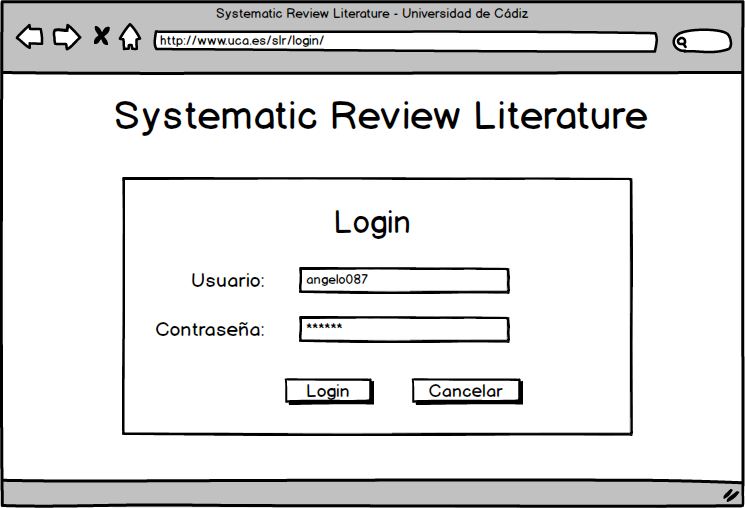
\includegraphics[scale=0.3]{mock01.png}
		\caption{Pantalla login.}
		\label{fig:mock01}
	\end{center}
\end{figure}

\begin{figure}[!hp]
	\begin{center} 
		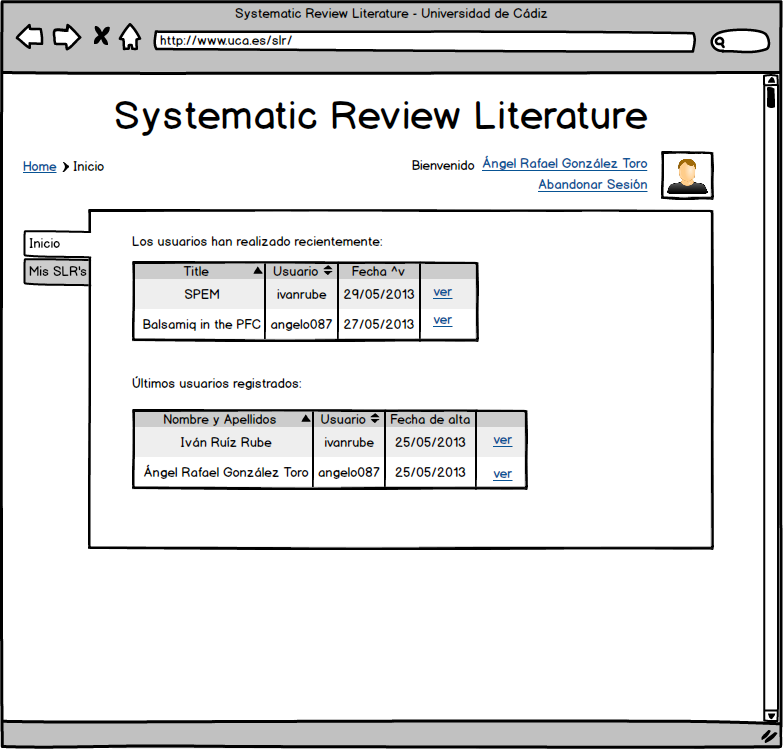
\includegraphics[scale=0.3]{mock02.png}
		\caption{Pantalla Revisiones Sistemáticas Usuario.}
		\label{fig:mock02}
	\end{center}
\end{figure}

\begin{figure}[!hp]
	\begin{center} 
		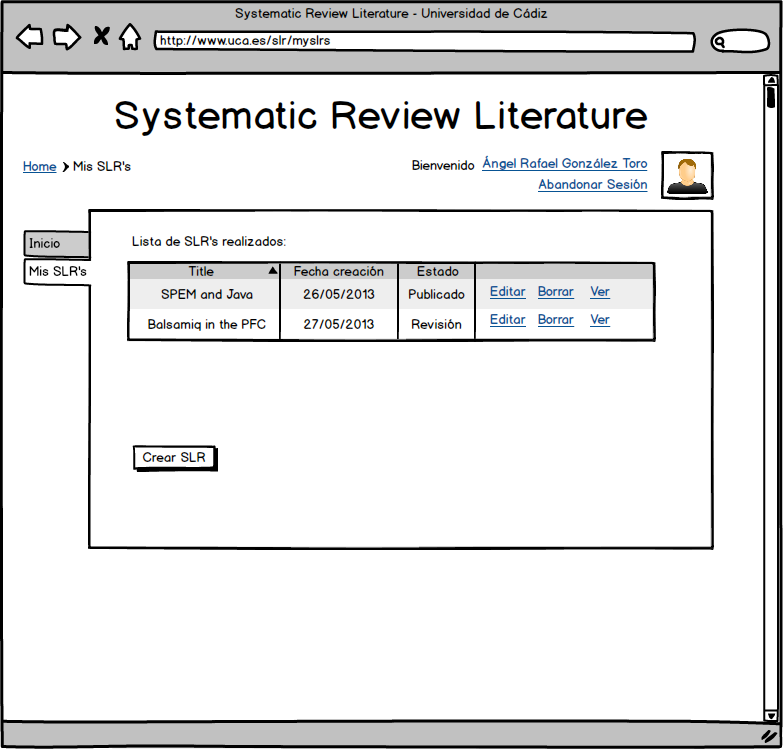
\includegraphics[scale=0.3]{mock03.png}
		\caption{Pantalla creación revisión sistemática}
		\label{fig:mock03}
	\end{center}
\end{figure}

\begin{figure}[!hp]
	\begin{center} 
		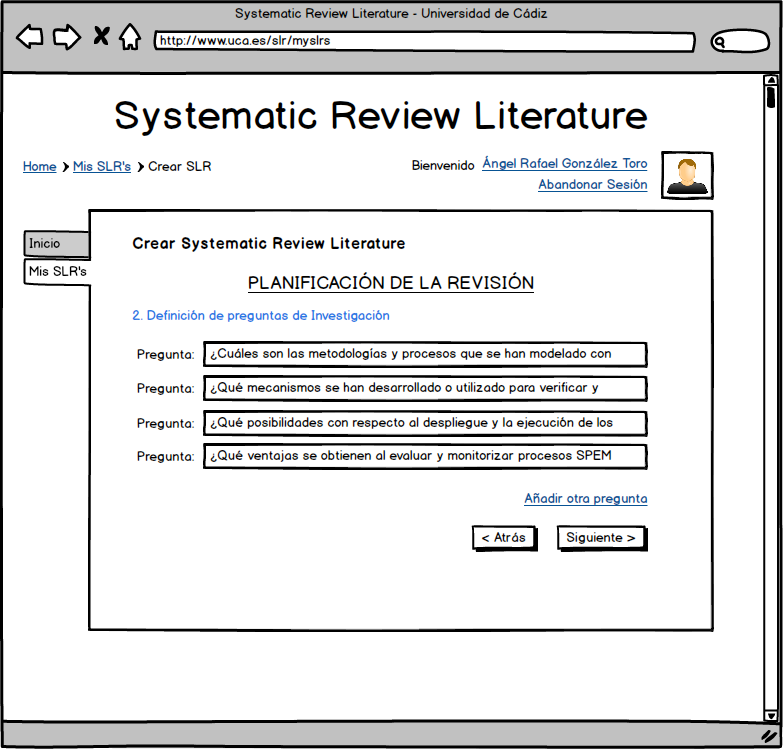
\includegraphics[scale=0.3]{mock04.png}
		\caption{Pantalla creación preguntas de investigación}
		\label{fig:mock04}
	\end{center}
\end{figure}

\begin{figure}[!hp]
	\begin{center} 
		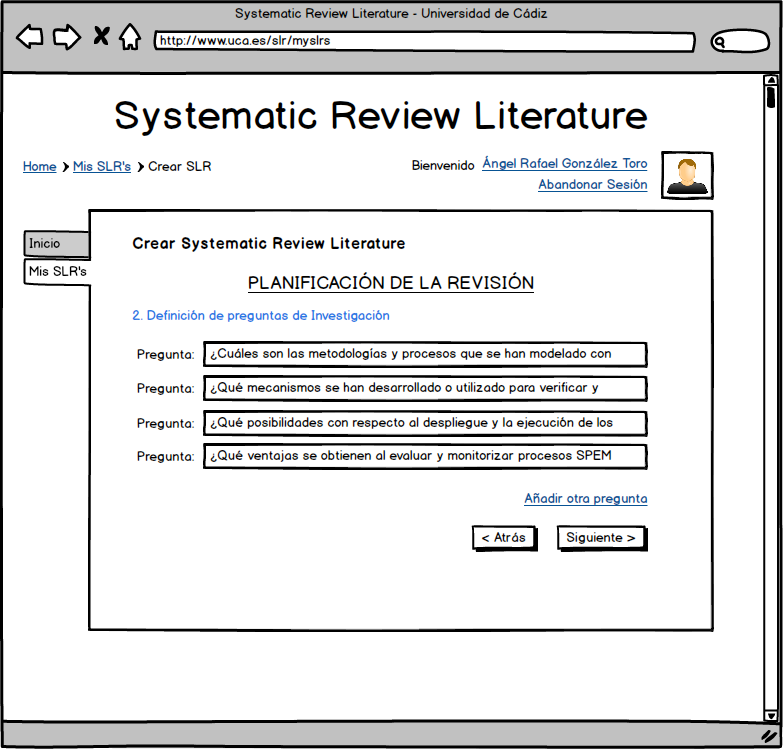
\includegraphics[scale=0.3]{mock05.png}
		\caption{Pantalla creación búsquedas de referencias bibliográficas.}
		\label{fig:mock05}
	\end{center}
\end{figure}

\begin{figure}[!hp]
	\begin{center} 
		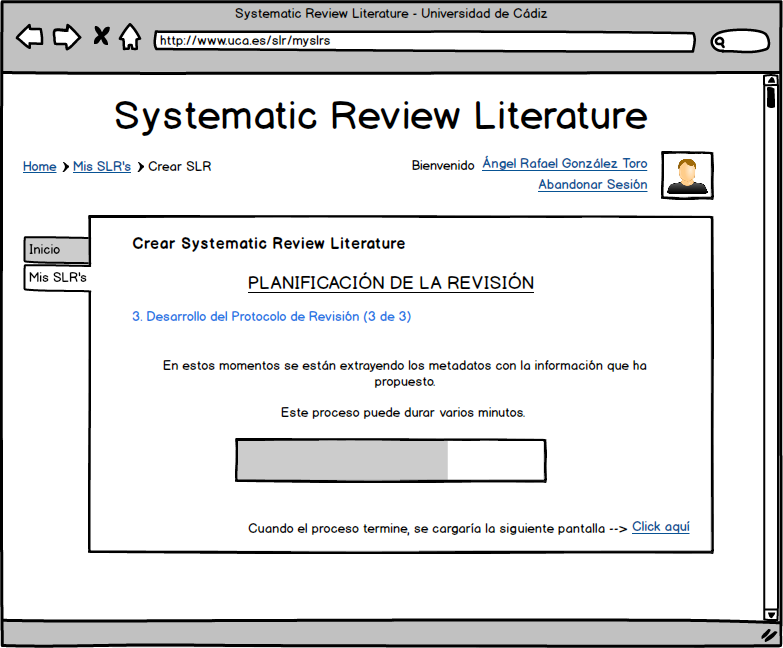
\includegraphics[scale=0.3]{mock06.png}
		\caption{Pantalla de creación de búsquedas en progreso.}
		\label{fig:mock06}
	\end{center}
\end{figure}

\begin{figure}[!hp]
	\begin{center} 
		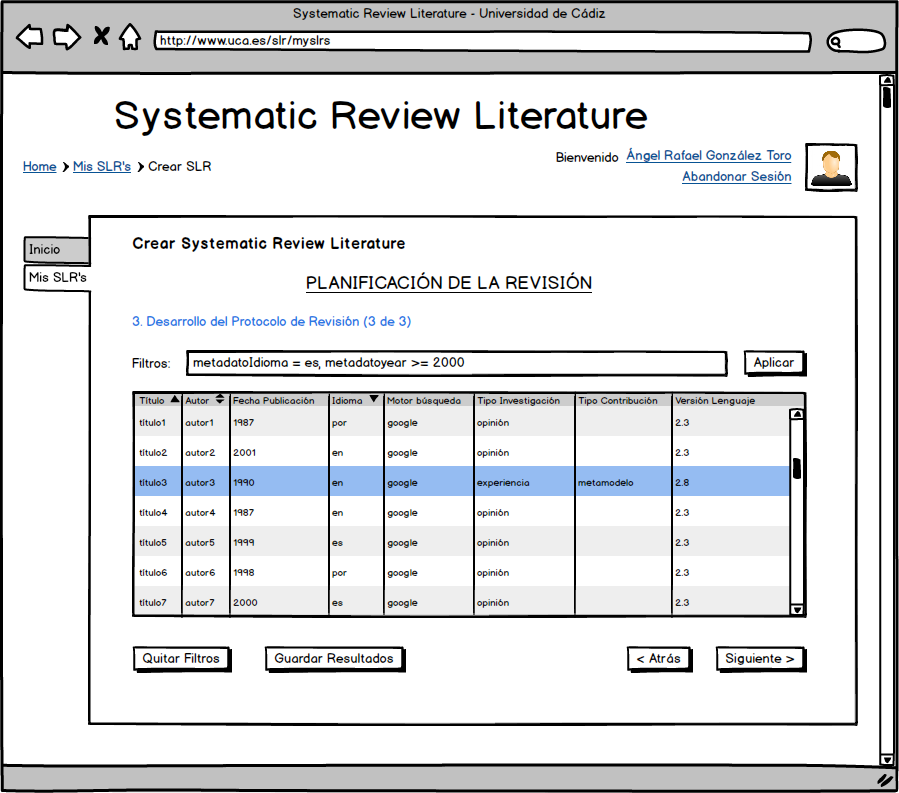
\includegraphics[scale=0.3]{mock07.png}
		\caption{Pantalla Referencias bibliográficas.}
		\label{fig:mock07}
	\end{center}
\end{figure}

\begin{figure}[!hp]
	\begin{center} 
		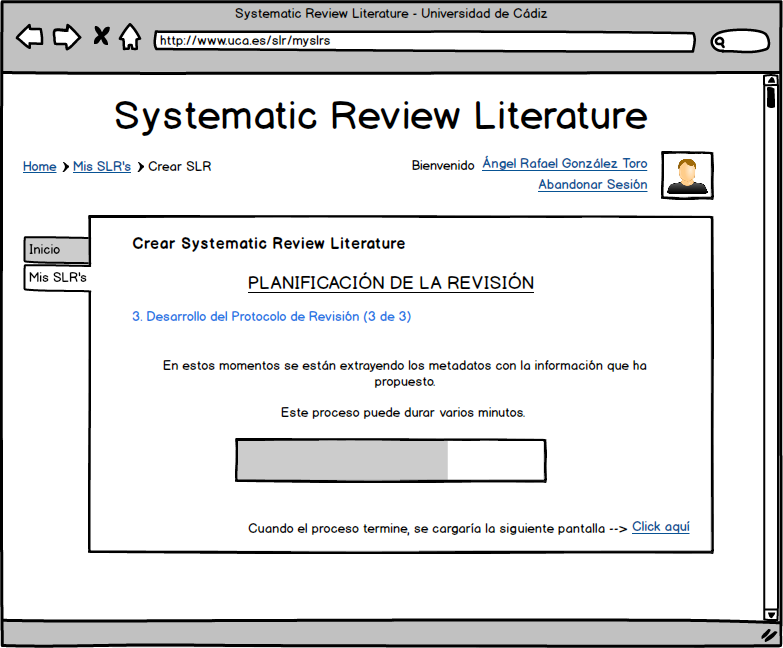
\includegraphics[scale=0.3]{mock08.png}
		\caption{Pantalla exportación referencias bibliográficas y gráficos (I).}
		\label{fig:mock08}
	\end{center}
\end{figure}

\begin{figure}[!hp]
	\begin{center} 
		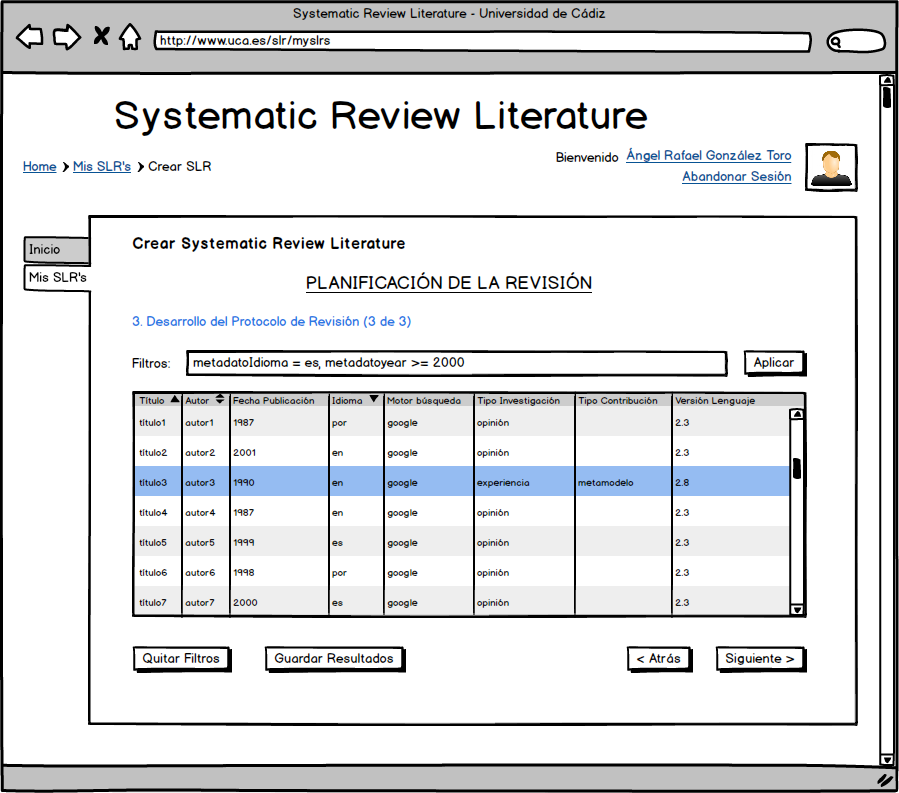
\includegraphics[scale=0.3]{mock09.png}
		\caption{Pantalla exportación referencias bibliográficas y gráficos (II).}
		\label{fig:mock09}
	\end{center}
\end{figure}

%En esta sección se deberá incluir un prototipo de baja fidelidad o mockup de la interfaz de usuario del sistema. Además, es preciso elaborar un diagrama de navegación, reflejando la secuencia de pantallas a las que tienen acceso los diferentes roles de usuario y la conexión entre éstas.
